% README file for moduleDocumentationTemplate TeX template.
% This template should be used to document all Basilisk modules.
% Updated 20170711 - S. Carnahan
%
%-Copy the contents of this folder to your own _Documentation folder
%
%-Rename the Basilisk-moduleDocumentationTemplate.tex appropriately
%
% All edits should be made in one of:
% sec_modelAssumptionsLimitations.tex
% sec_modelDescription.tex
% sec_modelFunctions.tex
% sec_revisionTable.tex
% sec_testDescription.tex
% sec_testParameters.tex
% sec_testResults.tex
% sec_user_guide.tex
%
%-Some rules about referencing within the document:
%1. If writing the user guide, assume the module description is present
%2. If writing the validation section, assume the module features section is present
%3. Make no other assumptions about any sections being present. This allow for sections of the document to be used elsewhere without breaking.

%In order to import some of these sections into a document in a different directory:
%\usepackage{import}
%Then, the sections are called with \subimport{relative path}{file} in order to \input{file} using the right relative path.
%\import{full path}{file} can also be used if absolute paths are preferred over relative paths.

%%%%%%%%%%%%%%%%%%%%%%%%%%%%%%%%%%%%%%%%%%%%%%%%%




\documentclass[]{BasiliskReportMemo}

\usepackage{cite}
\usepackage{AVS}
\usepackage{float} %use [H] to keep tables where you put them
\usepackage{array} %easy control of text in tables
\usepackage{graphicx}
\bibliographystyle{plain}


\newcommand{\submiterInstitute}{Autonomous Vehicle Simulation (AVS) Laboratory,\\ University of Colorado}


\newcommand{\ModuleName}{reactionWheelStateEffector}
\newcommand{\subject}{Reaction Wheel Dynamics Model}
\newcommand{\status}{To Be Reviewed}
\newcommand{\preparer}{C. Allard}
\newcommand{\summary}{The reaction wheel class is an instantiation of the state effector abstract class. The integrated test is validating the interaction between the reaction wheel module and the rigid body hub that it is attached to. More specifically, the reaction wheel module models three different cases: balanced wheels, simpled jitter, and fully coupled jitter. The details of each mode is described in detail in this document. There are integrated tests that confirm that all three models are agreeing with physics and the tests use both energy and momentum checks and back of the envelope (BOE) calculations. There are also unit tests verifying other functionality of the module}

\begin{document}

\makeCover

%
%	enter the revision documentation here
%	to add more lines, copy the table entry and the \hline, and paste after the current entry.
%
\pagestyle{empty}
{\renewcommand{\arraystretch}{2}
\noindent
\begin{longtable}{|p{0.5in}|p{3.5in}|p{1.07in}|p{0.9in}|}
\hline
{\bfseries Rev} & {\bfseries Change Description} & {\bfseries By}& {\bfseries Date} \\
\hline
1.0 & Initial Draft & C. Allard & 20170816\\
\hline
2.0 & Updated with new friction model & C. Allard & 20171120\\
\hline
\end{longtable}
}



\newpage
\setcounter{page}{1}
\pagestyle{fancy}

\tableofcontents %Autogenerate the table of contents
~\\ \hrule ~\\ %Makes the line under table of contents










	
\section{Model Description}

The gravity effector module is responsible for calculating the effects of gravity from a body on a spacecraft. A spherical harmonics model and implementation is developed and described below. The iterative methods used for the software algorithms are also described. Finally, the results of the code unit tests are presented and discussed.

\subsection{Relative Gravitational Dynamics Formulation}

The gravity effector module is critical to the propagation of spacecraft orbits in Basilisk. In order to increase the accuracy of spacecraft trajectories, a relative gravitational acceleration formulation can be used. Relative dynamics keep the acceleration, velocity, and distance magnitudes small, allowing more bits of a double variable to be used for accuracy, rather than magnitude. This additional accuracy is compounded via integration. This relative formulation is enforced when a user sets any planet in a multi-planet environment to have \verb|isCentralBody = True|.

If no planets in a simulation are set as the central body, then an absolute formulation of gravitational acceleration is used. In the absolute formulation, acceleration of a spacecraft due to each massive body is summed directly to calculate the resultant acceleration of the spacecraft.

\begin{equation}
	\ddot{\bm{r}}_{B/N, \mathrm{grav}} = \sum_{i = 1}^{n} \ddot{\bm{r}}_{B/N, i}
\end{equation}
where the accelerations on the right hand side are the acceleration due to the $i^{\mathrm{th}}$ planet which is being modeled as a gravity body. In this absolute mode, spacecraft position and velocity are integrated with respect to the inertial origin, typically solar system barycenter.

In the relative formulation, the acceleration of the spacecraft is calculated \textit{relative to} the central body. This is done by calculating the acceleration of the central body and subtracting it from the acceleration of the spacecraft.

\begin{equation}
	\ddot{\bm{r}}_{B/C, \mathrm{grav}} =\ddot{\bm{r}}_{B/N, \mathrm{grav}} - \ddot{\bm{r}}_{C/N, \mathrm{grav}}
\end{equation}

where $C$ is the central body. In this case, other accelerations of the central body (due to solar radiation pressure, for instance) are ignored.  For relative dynamics, the Basilisk dynamics integrator uses only \textit{relative} acceleration to calculate \textit{relative} position and velocity. The gravity module then accounts for this and modifies the spacecraft position and velocity by the central body's position and velocity after each timestep.

The above relative formulation leads to some questions regarding the accuracy of the dynamics integration. First, if acceleration due to gravity is being handled in a relative form, but accelerations due to external foces are handled absolutely, does Basilisk always produce the correct absolute position and velocity? Second, if dynamic state effectors such as hinged rigid bodies are using the gravitational acceleration that the spacecraft receives from the gravity module, are their states being integrated correctly?

Absolute accelerations (i.e. due to thrust) being integrated alongside the relative gravitational acceleration is handled easily due to the linearity of integration. In the absolute dynamics formulation there is:

\begin{equation}
	\ddot{\bm{r}}_{B/N} = \ddot{\bm{r}}_{B/N, \mathrm{grav}}  + \ddot{\bm{r}}_{B/N, \mathrm{thrust}} + \ddot{\bm{r}}_{B/N, \mathrm{SRP}} + \dots
	\label{eq:absGrav}
\end{equation}
and each term can be integrated separately on the right side so that
\begin{equation}
      \bm{r}_{B/N} = \int \int \ddot{\bm{r}}_{B/N, \mathrm{grav}} \mathrm{dtdt} +   \int \int \ddot{\bm{r}}_{B/N, \mathrm{thrust}} \mathrm{dtdt} +  \int \int \ddot{\bm{r}}_{B/N, \mathrm{SRP}}\mathrm{dt dt} +  \dots
\end{equation}
In the derivation that follows, the double integral to position is used, but the logic holds for the first integral to velocity as well. Now, because accelerations also add linearly,
\begin{equation}
\ddot{\bm{r}}_{B/N} = \ddot{\bm{r}}_{B/C} + \ddot{\bm{r}}_{C/N} = \ddot{\bm{r}}_{B/C, \mathrm{grav}} +  \ddot{\bm{r}}_{C/N, \mathrm{grav}}  + \ddot{\bm{r}}_{B/N, \mathrm{thrust}} + \ddot{\bm{r}}_{B/N, \mathrm{SRP}} + \dots
\end{equation}
which differs from Eq. \ref{eq:absGrav} in the gravitational acceleration of the spacecraft being split at the acceleration of the central body. Applying the integrals:
\begin{equation}
\bm{r}_{B/N} = \bm{r}_{B/C} + \bm{r}_{C/N} = \int \int \ddot{\bm{r}}_{B/C, \mathrm{grav}} \mathrm{dt dt} + \bm{r}_{C/N}  +   \int \int \ddot{\bm{r}}_{B/N, \mathrm{thrust}} \mathrm{dt dt} +  \int \int \ddot{\bm{r}}_{B/N, \mathrm{SRP}}\mathrm{dt dt} +  \dots
\end{equation}
where $\ddot{\bm{r}}_{C/N}$ is deliberately double integrated to $\bm{r}_{C/N}$ to show that it can be removed from both sides and $\bm{r}_{B/C}$ can be evaluated using relative gravitation acceleration combined with absolute accelerations due to external forces:
\begin{equation}
\bm{r}_{B/C}= \int \int \ddot{\bm{r}}_{B/C, \mathrm{grav}} \mathrm{dt dt} +   \int \int \ddot{\bm{r}}_{B/N, \mathrm{thrust}} \mathrm{dt dt} +  \int \int \ddot{\bm{r}}_{B/N, \mathrm{SRP}}\mathrm{dt dt} +  \dots
\end{equation}
Once that is done, it is clear that the absolute position can be found by simply adding the position of the central body to the relative position just found:
\begin{equation}
	\bm{r}_{B/N} = \bm{r}_{B/C} + \bm{r}_{C/N}
\end{equation}
This is how absolute position and velocity are found in Basilisk when using a relative dynamics formulation: the relative dynamics are integrated and the position and velocity of the central body are added afterward. The position and velocity of the central body are not integrated by Basilisk, but found from Spice.

Dynamic state effectors connected to the spacecraft hub can use the relative gravitational acceleration in their calculation for much the same reason. Effector positions and velocities are always integrated relative to the spacecraft. In fact, the absolute position and velocity of an effector is rarely, if ever, calculated or used. This is explains why a hinged body experiencing a relative acceleration does not quickly fall behind the spacecraft which is known to be moving along a course experiencing absolute gravitational acceleration. Additionally, because the effector is "pulled along" with the spacecraft when the spacecraft position is modified by the central body position, the effector sees the effect of absolute gravitational acceleration as well.

For intricacies related to using absolute vs relative dynamics, see the user manual at the end of this document.

\subsection{Spherical harmonics gravity model}

Gravity models are usually based on solutions of the Laplace equation ($\nabla^2 U(\mathbf{\bar r}) = 0$). It is very important to state that this equation only models a gravity potential outside a body. For computing a potential inside a body the Poisson equation is used instead.

The spherical harmonic potential is a solution of the Laplace equation using orthogonal spherical harmonics. It can be derived solving the Laplace equation in spherical coordinates, using the separation of variables technique and solving a Sturm-Liouville problem. In this work, the solution will be found using another technique, which essentially follows Vallado's book\cite{vallado2013}.

For each element of mass $d m_\text{Q}$ the potential can be written as
\begin{equation}
\D U(\mathbf{\bar r}) = G \frac{\D m_\text{Q}}{\rho_\text{Q}}
\end{equation}

where $\rho_\text{Q}$ is the distance between the element of mass and the position vector $\mathbf{\bar r}$ where the potential is computed. This position vector is usually given in a body-fixed frame. The relation between the position vector $\mathbf{\bar r}$, the position of the element of mass $\mathbf{\bar r_\text{Q}}$ and $\rho_\text{Q}$ can be given using the cosine theorem and the angle $\alpha$ between the two position vectors, as can be appreciated in Figure \ref{fig:spher_harm}.

\begin{figure}
	\centering
	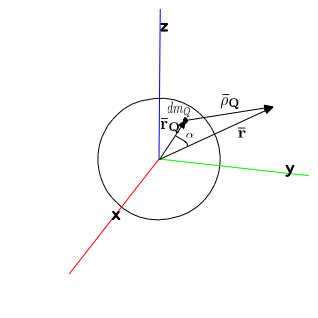
\includegraphics[width=0.3\textwidth]{Figures/spherical_harmonics.png}
	\caption{Geometry of the Spherical Harmonics Representation.}\label{fig:spher_harm}
\end{figure}

\begin{equation}
\rho_\text{Q} = \sqrt{r^2 + r_\text{Q}^2 - 2 r r_\text{Q} \cos(\alpha)} = r \sqrt{1 - 2 \frac{r_\text{Q}}{r} \cos(\alpha) + \bigg(\frac{r_\text{Q}}{r}\bigg)^2} = r \sqrt{1 - 2 \gamma \cos(\alpha) + \gamma^2}
\end{equation}
where $\gamma = r_\text{Q}/r$.

The potential can be obtained by integrating $dU$ through the whole body.
\begin{equation}
U(\mathbf{\bar r}) = G \int_{body} \frac{\D m_\text{Q}}{r \sqrt{1 - 2 \gamma \cos(\alpha) + \gamma^2}}
\end{equation}

If the potential is computed outside the body, $\gamma$ will always be less than 1, and the inverse of the square root can be approximated using the Legendre polynomials $P_l[\beta]$\cite{vallado2013}. Even though this derivation does not use the Laplace equation, it still assumes that the potential is computed outside the body.

The Legendre polynomials can be written as
\begin{equation}
P_l[\beta] = \frac{1}{2^l l!} \frac{d^l}{d \beta^l} (\beta^2 - 1)^l
\end{equation}

The potential is
\begin{equation}
U(\mathbf{\bar r}) = \frac{G}{r} \int_{body} \sum_{l=0}^\infty \gamma^l P_l[\cos(\alpha)] \D m_\text{Q}
\end{equation}

The angle $\alpha$ must be integrated. However, the cosine of the angle $\alpha$ can be decomposed using the geocentric latitude and the longitude associated to vectors $\mathbf{\bar r}$ and $\mathbf{\bar r_\text{Q}}$. These angles will be called $(\phi, \lambda)$ and $(\phi_\text{Q}, \lambda_\text{Q})$ respectively. Using the addition theorem it is possible to write\cite{vallado2013}.
\begin{equation}
P_l[cos(\alpha)] = P_l[\sin(\phi_\text{Q})] P_l[\sin(\phi)] + 2 \sum_{m=1}^l \frac{(l-m)!}{(l+m)!} (a_{l,m} a'_{l,m} + b_{l,m} b'_{l,m})
\end{equation}

where
\begin{align}
	a_{l,m} &= P_{l,m}[\sin(\phi_\text{Q})] \cos(m \lambda_\text{Q})\\
	b_{l,m} &= P_{l,m}[\sin(\phi_\text{Q})] \sin(m \lambda_\text{Q})\\
	a'_{l,m} &= P_{l,m}[\sin(\phi)] \cos(m \lambda)\\
	b'_{l,m} &= P_{l,m}[\sin(\phi)] \sin(m \lambda)
\end{align}

where $P_{l,m}[x]$ are the associated Legendre functions. "$l$" is called degree and "$m$", order. The polynomials can be computed as
\begin{equation}
P_{l,m}[\beta] = (1 - \beta^2)^\frac{m}{2} \frac{d^m}{d \beta^m} P_l[\beta]\label{eq:legendre}
\end{equation}

As can be seen, $a_{l,m}$ and $b_{l,m}$ must be integrated, but $a'_{l,m}$ and $a'_{l,m}$ can be taken outside the integral.
Therefore, it is possible to define
\begin{align}
	C'_{l,m} &= \int_{body} (2 -\delta_m) r_\text{Q}^l \frac{(l-m)!}{(l+m)!} a_{l,m} \D m_\text{Q}\\
	S'_{l,m} &= \int_{body} (2 -\delta_m) r_\text{Q}^l \frac{(l-m)!}{(l+m)!} b_{l,m} \D m_\text{Q}
\end{align}
where $\delta_m$ is the Kronecker delta.

Then
\begin{equation}
U(\mathbf{\bar r}) = \frac{G}{r} \sum_{l=0}^\infty C'_{l,0} \frac{P_l[\sin(\phi)]}{r^l} + \frac{G}{r} \sum_{l=0}^\infty \sum_{m=1}^l \frac{P_{l,m}[\sin(\phi)]}{r^l} \big[C'_{l,m} \cos(m \lambda) + S'_{l,m} \sin(m \lambda)]
\end{equation}

Non-dimensional coefficients $C_{l,m}$ and $S_{l,m}$ are usually used
\begin{align}
	C'_{l,m} &= C_{l,m} R_{\text{ref}}^l m_\text{Q}\\
	S'_{l,m} &= _\text{CoM}S_{l,m} R_{\text{ref}}^l m_\text{Q}
\end{align}
where $m_\text{Q}$ is the total mass of the body and $R_{\text{ref}}$ is a reference radius. If the coefficients $C_{l,m}$ and $S_{l,m}$ are given, the reference radius must be specified. Usually, the reference is chosen as the maximum radius or the mean radius\cite{scheeres2012}.

The potential is then
\begin{equation}
U(\mathbf{\bar r}) = \frac{\mu}{r} \sum_{l=0}^\infty C_{l,0} \bigg(\frac{R_{\text{ref}}}{r}\bigg)^l P_l[\sin(\phi)] + \frac{\mu}{r} \sum_{l=0}^\infty \sum_{m=1}^l \bigg(\frac{R_{\text{ref}}}{r}\bigg)^l P_{l,m}[\sin(\phi)] \big[C_{l,m} \cos(m \lambda) + S_{l,m} \sin(m \lambda)\big]
\end{equation}

Since $P_l[x] = P_{l,0}[x]$ the potential can be written in a more compact way
\begin{equation}
U(\mathbf{\bar r}) = \frac{\mu}{r} \sum_{l=0}^\infty \sum_{m=0}^l \bigg(\frac{R_{\text{ref}}}{r}\bigg)^l P_{l,m}[\sin(\phi)] \big[C_{l,m} \cos(m \lambda) + S_{l,m} \sin(m \lambda)\big]
\end{equation}

Some coefficients have a very interesting interpretation. 
\begin{align}
	C_{0,0} &= 1\\
	S_{l,0} &= 0 \quad \forall l \geq 0\\
	C_{1,0} &= \frac{Z_{\text{CoM}}}{R_{\text{ref}}}\\
	C_{1,1} &= \frac{X_{\text{CoM}}}{R_{\text{ref}}}\\
	S_{1,1} &= \frac{Y_{\text{CoM}}}{R_{\text{ref}}}
\end{align}

where $[X_\text{CoM}, Y_\text{CoM}, Z_\text{CoM}]$ represents the center of mass of the celestial body. Therefore, if the origin of the coordinate system coincides with the center of mass, all these coefficients are identically zero. Similarly, the second order coefficients are related to the second order moments (moments of inertia).

Finally, the coefficients and Legendre polynomials are usually normalized to avoid computational issues. The factor $N_{l,m}$ is called the normalization factor
\begin{equation}
N_{l,m} = \sqrt{\frac{(l-m)! (2 -\delta_m) (2 l +1)}{(l+m)!}}
\end{equation}

The normalized coefficients are
\begin{align}
	\bar C_{l,m} &= \frac{C_{l,m}}{N_{l,m}}\\
	\bar S_{l,m} &= \frac{S_{l,m}}{N_{l,m}}
\end{align}

The normalized associated Legendre functions are
\begin{equation}
\bar P_{l,m}[x] = P_{l,m}[x] N_{l,m}
\end{equation}

The potential may be written as
\begin{equation}
U(\mathbf{\bar r}) = \frac{\mu}{r} \sum_{l=0}^\infty \sum_{m=0}^l \bigg(\frac{R_{\text{ref}}}{r}\bigg)^l \bar P_{l,m}[\sin(\phi)] \big[\bar C_{l,m} \cos(m \lambda) + \bar S_{l,m} \sin(m \lambda)\big]
\end{equation}

\subsubsection{Pines' Representation of Spherical Harmonics Gravity}

There are many ways to algorithmically compute the potential and its first and secondary derivatives. One of such algorithms is the one proposed by Pines\cite{pines1973}.

The spherical harmonics representation as it was presented has a singularity at the poles for the gravity field. The Pines' formulation avoids this problem and is more numerically stable for high degree and high order terms.

Unfortunately, this formulation does not contain the normalization factor which is necessary if the coefficients are normalized. In a paper written by Lundberg and Schutz\cite{lundberg1988}, a normalized representation of the Pines' formulation is given, but it contains an approximation.

For this work, and in order to code the spherical harmonics formulation, a formulation similar to Pines' using the Lundberg-Schutz paper will be derived. However, no approximations will be used. Therefore, the algorithm will be developed here without using the exact formulations given in those papers. For the sake of brevity, not every single derivation will be carried out, but it is possible to get the results following the expressions obtained in this section.

In the Pines' formulation the radius and the director cosines are used as coordinates. The potential will be given as $U[r, s, t, u]$, where
\begin{align}
	r &= \sqrt{x^2+y^2+z^2}\\
	s &= \frac{x}{r}\\
	t &= \frac{y}{r}\\
	u &= \frac{z}{r}
\end{align}

For a function of these coordinates, the dependance will be given using square brackets (e.g. $f[r,s,t,u]$).

Since $u = \sin(\phi) = \cos(90^\circ - \phi)$, it is possible to write
\begin{equation}
P_{l,m}[\sin(\phi)] = P_{l,m}[u]
\end{equation}

The derived Legendre functions $A_{l,m}[u]$ are defined such that
\begin{equation}
P_{l,m}[u] = (1 - u^2)^\frac{m}{2} A_{l,m}[u]
\end{equation}

From the definition of $P_{l,m}$ (Equation \refeq{eq:legendre}), it is possible to write
\begin{equation}
A_{l,m}[u] = \frac{d^m}{d u^m} P_l[u] = \frac{1}{2^l l!} \frac{d^{l+m}}{d u^{l+m}} (u^2 - 1)^l\label{eq:der_leg}
\end{equation}

The term $(1 - u^2)^\frac{m}{2}$ can be written as $(1 - \sin^2(\phi))^\frac{m}{2} = |\cos(\phi)|^m = \cos^m(\phi)$.

If the complex number $\xi$ is defined such that ($j$ is the imaginary unit)
\begin{equation}
\xi = \cos(\phi) \cos(\lambda) + j \cos(\phi) \sin(\lambda) = \frac{x}{r} + j \frac{y}{r} = s + j t
\end{equation}

it is possible to write
\begin{equation}
\xi^m = \cos^m(\phi) e^{j m \lambda} = (s + j t)^m
\end{equation}

The following sequences may be defined
\begin{align}
	R_m[s,t] &= Re\{\xi^m\}\\
	I_m[s,t] &= Im\{\xi^m\}
\end{align}

Putting all together, it is possible to write
\begin{equation}
U(\mathbf{\bar r}) = \frac{\mu}{r} \sum_{l=0}^\infty \sum_{m=0}^l \bigg(\frac{R_{\text{ref}}}{r}\bigg)^l A_{l,m}[u] \{C_{l,m} R_m[s,t] + S_{l,m} I_m[s,t]\}
\end{equation}

In order to normalize the coefficients ($\bar C_{l,m}$ and $\bar S_{l,m}$) and the derived Legendre functions ($\bar A_{l,m} = N_{l,m} A_{l,m}$), each term is divided an multiplied by the normalization factor $N_{l,m}$. Then
\begin{equation}
U(\mathbf{\bar r}) = \frac{\mu}{r} \sum_{l=0}^\infty \sum_{m=0}^l \bigg(\frac{R_{\text{ref}}}{r}\bigg)^l \bar A_{l,m}[u] \{\bar C_{l,m} R_m[s,t] + \bar S_{l,m} I_m[s,t]\}
\end{equation}

The sets $D_{l,m}[s,t]$, $E_{l,m}[s,t]$, and $F_{l,m}[s,t]$, are defined as
\begin{align}
	D_{l,m}[s,t] &= \bar C_{l,m} R_m[s,t] + \bar S_{l,m} I_m[s,t]\\
	E_{l,m}[s,t] &= \bar C_{l,m} R_{m-1}[s,t] + \bar S_{l,m} I_{m-1}[s,t]\\
	F_{l,m}[s,t] &= \bar S_{l,m} R_{m-1}[s,t] - \bar C_{l,m} I_{m-1}[s,t]
\end{align}

The value $\rho_l[r]$ is also defined as
\begin{equation}
\rho_l[r] = \frac{\mu}{r} \bigg(\frac{R_{\text{ref}}}{r}\bigg)^l
\end{equation}

The gravity potential may be finally computed as
\begin{equation}
U(\mathbf{\bar r}) = \sum_{l=0}^\infty \sum_{m=0}^l \rho_l[r] \bar A_{l,m}[u] D_{l,m}[s,t]
\end{equation}

This is the final expression that will be used to compute the gravity potential.

\subsubsection{Recursion Formulas}

Several recursion formulas are needed in order to algorithmically implement the Pines' formulation. They will be given without proof, but they are easily derived using the definitions above.
\begin{itemize}


\item{Recursion formula for $\rho_l[r]$}

Initial condition: $\rho_0[r] = \frac{\mu}{r}$
\begin{equation}
\rho_l[r] = \rho \cdot \rho_{l-1}[r]
\end{equation}
where $\rho = R_{\text{ref}}/r$.

\item{Recursion formula for $R_m[s,t]$}

Initial condition: $R_0[s,t] = 1$
\begin{equation}
R_m[s,t] = s R_{m-1}[s,t] - t I_{m-1}[s,t]
\end{equation}

\item{Recursion formula for $I_m[s,t]$}

Initial condition: $I_0[s,t] = 0$
\begin{equation}
I_m[s,t] = s I_{m-1}[s,t] + t R_{m-1}[s,t]
\end{equation}

\item{Recursion formula for $\bar A_{l,m}[u]$}

From Equation \eqref{eq:der_leg}, it is possible to see that
\begin{align}
	A_{l,l}[u] &= (2 l -1) A_{l-1,l-1}[u]\label{eq:All}\\
	A_{l,l-1}[u] &= u A_{l,l}[u]\label{eq:All_1}
\end{align}
\end{itemize}
There are several recursion formulas for computing Legendre polynomials $A_{l,m}[u]$, for $m < l-1$. The following formula, which is stable for high degrees\cite{lundberg1988}, will be used:
\begin{equation}
A_{l,m}[u] = \frac{1}{l-m} ((2 l -1) u A_{l-1,m}[u] - (l+m-1) A_{l-2,m}[u])\label{eq:Alm}
\end{equation}

Using Equations \eqref{eq:All}, \eqref{eq:All_1}, and \eqref{eq:Alm}, and the definition $\bar A_{l,m}[u] = N_{l,m} A_{l,m}[u]$, the following recursion formulas can be derived.

Initial condition: $\bar A_{0,0}[u] = 1$

The diagonal terms are computed as
\begin{equation}
\bar A_{l,l}[u] = \sqrt{\frac{(2 l - 1) (2 - \delta_l)}{(2 l) (2 - \delta_{l-1})}} \bar A_{l-1,l-1}[u]
\end{equation}

The low diagonal terms are then calculated as
\begin{equation}
\bar A_{l,l-1}[u] = u \sqrt{\frac{(2 l) (2 - \delta_{l-1})}{2 - \delta_l}} \bar A_{l,l}[u]
\end{equation}

Finally, for $l \geq (m+2)$, $N1_{l,m}$ and $N2_{l,m}$ are defined such that
\begin{align}
	N1_{l,m} &= \sqrt{\frac{(2 l + 1) (2 l - 1)}{(l - m) (l + m)}}\\
	N2_{l,m} &= \sqrt{\frac{(l + m - 1) (2 l + 1) (l - m -1)}{(l - m) (l + m) (2 l - 3)}}
\end{align}

and $\bar A_{l,m}[u]$ computed using

\begin{equation}
\bar A_{l,m}[u] = u N1_{l,m} \bar A_{l-1,m}[u] - N2_{l,m} \bar A_{l-2,m}[u]
\end{equation}


\subsubsection{Derivatives}

The first order derivatives of many of the values given are necessary to compute the gravity field (second order derivatives are needed if the Hessian is to be computed).

It is easy to show that
\begin{align}
	\frac{\partial D_{l,m}}{\partial s}[s,t] &= m E_{l,m}[s,t]\\
	\frac{\partial D_{l,m}}{\partial t}[s,t] &= m F_{l,m}[s,t]
\end{align}

\begin{equation}
\frac{d \rho_l}{d r}[r] = -\frac{(l+1)}{R_{\text{ref}}} \rho_{l+1}[r]
\end{equation}

\begin{align}
	\frac{\partial R_m}{\partial s}[s,t] &= m R_{m-1}[s,t]\\
	\frac{\partial R_m}{\partial t}[s,t] &= -m I_{m-1}[s,t]\\
	\frac{\partial I_m}{\partial s}[s,t] &= m I_{m-1}[s,t]\\
	\frac{\partial I_m}{\partial t}[s,t] &= m R_{m-1}[s,t]
\end{align}

\begin{equation}
\frac{d \bar A_{l,m}}{d u}[u] = \frac{N_{l,m}}{N_{l,m+1}} \bar A_{l,m+1}[u]
\end{equation}

The gravity field can be computed using all the equations given. However, the gradient of the potential is needed. As a change of variables was realized, the chain rule must be applied. In order to avoid filling up pages with math derivations, the results will be given. With patience, the following results can be obtained applying the chain rule and using all the derivatives given.

The gravity field can be computed as
\begin{equation}
\mathbf{\bar g} = (a_1[r,s,t,u] + s \cdot a_4[r,s,t,u]) \mathbf{\hat i} + (a_2[r,s,t,u] + t \cdot a_4[r,s,t,u]) \mathbf{\hat j} + (a_3[r,s,t,u] + u \cdot a_4[r,s,t,u]) \mathbf{\hat k}
\end{equation}

where
\begin{align}
	a_1[r,s,t,u] &= \sum_{l=0}^\infty \sum_{m=0}^l \frac{\rho_{l+1}[r]}{R_{\text{ref}}} m \bar A_{l,m}[u] E_{l,m}[s,t]\\
	a_2[r,s,t,u] &= \sum_{l=0}^\infty \sum_{m=0}^l \frac{\rho_{l+1}[r]}{R_{\text{ref}}} m \bar A_{l,m}[u] F_{l,m}[s,t]\\
	a_3[r,s,t,u] &= \sum_{l=0}^\infty \sum_{m=0}^l \frac{\rho_{l+1}[r]}{R_{\text{ref}}} m \frac{N_{l,m}}{N_{l,m+1}} \bar A_{l,m+1}[u] D_{l,m}[s,t]\\
	a_4[r,s,t,u] &= \sum_{l=0}^\infty \sum_{m=0}^l \frac{\rho_{l+1}[r]}{R_{\text{ref}}} m \frac{N_{l,m}}{N_{l+1,m+1}} \bar A_{l+1,m+1}[u] D_{l,m}[s,t]
\end{align}

In order to avoid computing factorials, it is easy to see that
\begin{align}
	\frac{N_{l,m}}{N_{l,m+1}} &= \sqrt{\frac{(l-m) (2-\delta_m)(l+m+1)}{2- \delta_{m+1}}}\\
	\frac{N_{l,m}}{N_{l+1,m+1}} &= \sqrt{\frac{(l+m+2)(l+m+1)(2l+1)(2-\delta_m)}{(2l+3)(2-\delta_{m+1})}}
\end{align}

Using all these expressions, the potential and the gravity field can be computed.

\subsection{Polyhedral gravity model}

The polyhedral model, described in Werner and Scheeres publication\cite{werner1996} , computes the exterior gravity of a polyhedron with constant density $\sigma$. Let recall that a polyhedron is geometrically described by a number of planar faces composed by vertexes. An edge $e$ is the line connecting two adjacent vertexes belonging to the same face $f$ (the edges follow a counterclockwise concatenation). The potential of such object is

\begin{equation}
U(\bar{\mathbf{r}})=- \frac{1}{2}G\sigma\sum_{f\in\text{faces}}\left(\mathbf{r}_f \cdot\mathbf{n}_f\mathbf{n}_f\cdot\mathbf{r}_f\omega_f-\sum_{e\in\text{face's edges}}\mathbf{r}_f\cdot\mathbf{n}_f\mathbf{n}_e\cdot\mathbf{r}_e L_e\right)\label{eq:polyhedral_potential}
\end{equation}

 The vector $\mathbf{r}_f$ extends from the evaluation point to any vertex on the face. The variable $\mathbf{n}_f$ is the outward-pointing normal vector of face $f$. The term $\omega_f$ is the signed solid angle subtended by the face $f$ when viewed from the evalution point. The variable $\mathbf{r}_e$ is a vector from the evaluation point to the initial vertex of edge $e$. The vector $\mathbf{n}_e$ is the normal of the edge lying on the face plane. The term $L_e$ corresponds to the potential of a 1D wire.
 
 Note that in Werner and Scheeres\cite{werner1996}, the double summation term of \eqref{eq:polyhedral_potential} was simplified to a single summation over all polyhedron's edges. Although that reduction is convenient for mathematical compactness, retaining the double summation simplifies the algorithmic implementation (so that there is no need to check for common edges between adjacent faces).
 
 In order to provide consistency with other gravity models, the density $\sigma$ is computed based on the polyhedron shape and the input gravity parameter $\mu$. The volume of a trisurface polyhedron is
 \begin{equation}
 V = \frac{1}{6}\sum_{f\in\text{faces}}|(\mathbf{r}^{f}_1\times\mathbf{r}^{f}_2)\cdot \mathbf{r}^{f}_3|,
 \end{equation}
then $\sigma=\mu / (VG)$. The vector $\mathbf{r}^{f}_i$, $i=1,2,3$, is the position of each face's vertex.

\subsection{Point Mass Gravity}
The point mass gravity model is equivalent to using only the $0^{\text{th}}$ term of the spherical harmonics equations. This is the equation that is used in basics physics courses and is most often used in Basilisk simulations. It assumes the gravitational body to be a point mass:

\begin{equation}
U(\mathbf{\bar r}) = G \frac{ m_\text{Q}}{\rho_\text{Q}}
\end{equation}
 %This section includes mathematical models, code description, etc.

\section{Model Functions}
The mathematical description of the IMU are implemented in imu\_sensor.cpp. This code performs the following primary functions
\begin{itemize}
	\item \textbf{Spacecraft State Measurement}: The code provides measurements of the spacecraft state (angular and linear).
	\item \textbf{Bias Modeling}: The code adds instrument bias and bias random walk to the signals.
	\item \textbf{Noise Modeling}: The code calculates noise according to the Gauss Markov model if the user asks for it and provides a perturbation matrix.
	\item \textbf{Discretization}: The code discretizes the signal to emulate real digital instrumentation. The least significant bit (LSB, sensor resolution) can be set by the user.
	\item \textbf{Saturation}: The code bounds the output signal according to user-specified maximum and minimum saturation values.
	\item \textbf{Accelerometer Center of Mass Offset}: The code can handle accelerometer placement other than the center of mass of the spacecraft.
	\item \textbf{Scale Factor}: The code can apply a scale factor, different for each axis of acceleration and angular rate, to the measured value (truth + noise + bias). This is a linear scaling of the output.
	\item \textbf{Bias Random Walk Bounds}: The code bounds bias random walk per user-specified bounds.
	\item \textbf{Interface: Spacecraft States}: The code sends and receives spacecraft state information via the Basilisk messaging system.
\end{itemize}


\section{Model Assumptions and Limitations}
This code makes assumptions which are common to IMU modeling.
\begin{itemize}
	\item \textbf{Error Inputs}: Because the error models rely on user inputs, these inputs are the most likely source of error in IMU output. Instrument bias would have to be measured experimentally or an educated guess would have to be made. The Guass-Markov noise model has well-known assumptions and is generally accepted to be a good model for this application.
	\item \textbf{Error Integration}: Errors for integrated values (DV and PRV) are calculated as acceleration and angular velocity errors multiplied by the IMU time step.  If the IMU timestep matches the dynamics process rate, this is possibly a good assumption. However, if the IMU is run slower than the dynamics process, then the velocity errors may not be related to the instantaneous acceleration errors at the sampling time.
	
	\item \textbf{Integral Saturation}: Because the DV and PRV output values are calculated only at the IMU time step and not actually by integrating rates multiple times between calls, their saturation values are taken as the time integral of the rate saturation values. This misses some possibilities with varying accelerations between IMU time steps. Furthermore, the PRV is taken to be the integral of the angular rate over the time step. This should be a good approximation if the attitude of the spacecraft doesn't change "too much" over a relevant time step.
	
	\item \textbf{IMU Rate Limitation}: As with a real IMU, this model will only be run at a finite speed. It is limited in that it cannot correctly capture dynamics that are happening much faster than the IMU is called. 
\end{itemize} %This includes a concise list of what the module does. It also includes model assumptions and limitations

% !TEX root = ./Basilisk-MRPROTATION-20180522.tex

\section{Test Description and Success Criteria}
The module is run on its own with specified inputs to ensure the outputs are correct.  The outputs are evaluated dynamically using a support python script, and then compared to the Basilisk evaluated results.  A nominal simulation length of 1 second is used with a time step of 0.5 seconds, yielding 3 return values.

If the rotation states are set directly in the module by specifying {\tt mrpSet} and {\tt omega\_RR0\_R}, then the values $\bm\sigma_{R/R_{0}}(t_{0}) = $[0.3 0.5 0. ] and $\leftexp{R}{\bm\omega}_{R/R_{0}}=$[0.1 0.  0. ]deg/sec are used.  The simulation flag {\tt cmdStateFlag} determines if the rotation states are specified through an input message.  If yes, then the values $\bm\sigma_{R/R_{0}}(t_{0}) = $[ 0.1  0.  -0.2] and $\leftexp{R}{\bm\omega}_{R/R_{0}}=$[0.1 1.  0.5]deg/sec are used instead.  

If the simulation flag {\tt stateOutputFlag} is true then  the optional attitude states of $\mathcal{R}$ relative to $\mathcal{R}_{0}$ are provided in an output message.

If the simulation flag {\tt testReset} is true then  the simulation will run an addition 1 second, but after a reset function is called.

\begin{table}[htbp]
	\caption{Test Scenarios.}
	\label{tab:checks}
	\centering \fontsize{10}{10}\selectfont
	\begin{tabular}{ l | c | c | c } % Column formatting, 
		\hline\hline
		\textbf{Check}  & {\tt cmdStateFlag} & {\tt testReset}  \\ 
		\hline
		1 & False  & False \\
		2 & True  & False \\
		3 & False  & True \\
		4 & True  & True \\
		\hline\hline
	\end{tabular}
\end{table}

\section{Test Parameters}
The output variables being tested are listed in Table~\ref{tab:errortol}, including the test tolerance value.

\begin{table}[htbp]
	\caption{Error tolerance for each test.}
	\label{tab:errortol}
	\centering \fontsize{10}{10}\selectfont
	\begin{tabular}{ c | c } % Column formatting, 
		\hline\hline
		\textbf{Output Value Tested}  & \textbf{Tolerated Error}  \\ 
		\hline
		{\tt attRefOutMsg.sigma\_RN}        & 1e-10	   \\
		{\tt attRefOutMsg.omega\_RN\_N}        & 1e-10	   \\
		{\tt attRefOutMsg.domega\_RN\_N}        & 1e-10	   \\
		{\tt attitudeOutMsg.state}        & 1e-10	   \\
		{\tt attitudeOutMsg.rate}        & 1e-10	   \\
		\hline\hline
	\end{tabular}
\end{table}




\section{Test Results}
The results of the unit test are listed in Table~\ref{tab:results}.  
All of the tests are expected to pass:
\begin{table}[H]
	\caption{Test results}
	\label{tab:results}
	\centering \fontsize{10}{10}\selectfont
	\begin{tabular}{c | c  } % Column formatting, 
		\hline\hline
		\textbf{Check} 						  		&\textbf{Pass/Fail} \\ 
		\hline
	   1	   			& \textcolor{ForestGreen}{PASSED} \\ 
	   2	   			& \textcolor{ForestGreen}{PASSED} \\ 
	   3	   			& \textcolor{ForestGreen}{PASSED} \\ 
	   4	   			& \textcolor{ForestGreen}{PASSED} \\ 
	   \hline\hline
	\end{tabular}
\end{table}


 % This includes test description, test parameters, and test results

% !TEX root = ./Basilisk-inertialUKF-20190402.tex

\section{User Guide}
\subsection{Filter Set-up, initialization, and I/O}

In order for the filter to run, the user must set a few parameters:

\begin{itemize}
\item The unscented filter has 3 parameters that need to be set, and are best as: \\
      \texttt{ filterObject.alpha = 0.02} \\
      \texttt{ filterObject.beta = 2.0} \\
      \texttt{ filterObject.kappa = 0.0} 
\item Initialize orbit: \\ 
\texttt{     mu = 42828.314*1E9 \#m3/s2} \\
 \texttt{    elementsInit = orbitalMotion.ClassicElements()} \\
 \texttt{    elementsInit.a = 4000*1E3 \#meters} \\
 \texttt{    elementsInit.e = 0.2} \\
 \texttt{    elementsInit.i = 10} \\
  \texttt{   elementsInit.Omega = 0.001} \\
 \texttt{    elementsInit.omega = 0.01} \\
 \texttt{    elementsInit.f = 0.1} \\
 \texttt{    r, v = orbitalMotion.elem2rv(mu, elementsInit)} 
\item The initial covariance: \\
 \texttt{Filter.covar =} \\
  \texttt{[1000*1E6, 0.0, 0.0, 0.0, 0.0, 0.0,\\
                              0.0, 1000.*1E6, 0.0, 0.0, 0.0, 0.0,\\
                              0.0, 0.0, 1000.*1E6, 0.0, 0.0, 0.0,\\
                              0.0, 0.0, 0.0, 5.*1E6, 0.0, 0.0,\\
                              0.0, 0.0, 0.0, 0.0, 5.*1E6, 0.0,\\
                              0.0, 0.0, 0.0, 0.0, 0.0, 5.*1E6]}
 \item The initial state :\\
  \texttt{      filterObject.stateInit = r.tolist() + v.tolist()} 
    \item The process noise :\\
  \texttt{     qNoiseIn = np.identity(6)} \\
  \texttt{     qNoiseIn[0:3, 0:3] = qNoiseIn[0:3, 0:3]*1E-8*1E-8} \\
  \texttt{     qNoiseIn[3:6, 3:6] = qNoiseIn[3:6, 3:6]*1E7*1E7} \\
  \texttt{     filterObject.qNoise = qNoiseIn.reshape(36).tolist()}
\end{itemize}

 % Contains a discussion of how to setup and configure  the BSK module







\bibliography{bibliography} %This includes references used and mentioned.

\end{document}
